% Options for packages loaded elsewhere
\PassOptionsToPackage{unicode}{hyperref}
\PassOptionsToPackage{hyphens}{url}
%
\documentclass[
]{book}
\usepackage{amsmath,amssymb}
\usepackage{lmodern}
\usepackage{iftex}
\ifPDFTeX
  \usepackage[T1]{fontenc}
  \usepackage[utf8]{inputenc}
  \usepackage{textcomp} % provide euro and other symbols
\else % if luatex or xetex
  \usepackage{unicode-math}
  \defaultfontfeatures{Scale=MatchLowercase}
  \defaultfontfeatures[\rmfamily]{Ligatures=TeX,Scale=1}
\fi
% Use upquote if available, for straight quotes in verbatim environments
\IfFileExists{upquote.sty}{\usepackage{upquote}}{}
\IfFileExists{microtype.sty}{% use microtype if available
  \usepackage[]{microtype}
  \UseMicrotypeSet[protrusion]{basicmath} % disable protrusion for tt fonts
}{}
\makeatletter
\@ifundefined{KOMAClassName}{% if non-KOMA class
  \IfFileExists{parskip.sty}{%
    \usepackage{parskip}
  }{% else
    \setlength{\parindent}{0pt}
    \setlength{\parskip}{6pt plus 2pt minus 1pt}}
}{% if KOMA class
  \KOMAoptions{parskip=half}}
\makeatother
\usepackage{xcolor}
\IfFileExists{xurl.sty}{\usepackage{xurl}}{} % add URL line breaks if available
\IfFileExists{bookmark.sty}{\usepackage{bookmark}}{\usepackage{hyperref}}
\hypersetup{
  pdftitle={Machine Learning for Quantitative Investment},
  pdfauthor={Fintelligence},
  hidelinks,
  pdfcreator={LaTeX via pandoc}}
\urlstyle{same} % disable monospaced font for URLs
\usepackage{color}
\usepackage{fancyvrb}
\newcommand{\VerbBar}{|}
\newcommand{\VERB}{\Verb[commandchars=\\\{\}]}
\DefineVerbatimEnvironment{Highlighting}{Verbatim}{commandchars=\\\{\}}
% Add ',fontsize=\small' for more characters per line
\usepackage{framed}
\definecolor{shadecolor}{RGB}{248,248,248}
\newenvironment{Shaded}{\begin{snugshade}}{\end{snugshade}}
\newcommand{\AlertTok}[1]{\textcolor[rgb]{0.94,0.16,0.16}{#1}}
\newcommand{\AnnotationTok}[1]{\textcolor[rgb]{0.56,0.35,0.01}{\textbf{\textit{#1}}}}
\newcommand{\AttributeTok}[1]{\textcolor[rgb]{0.77,0.63,0.00}{#1}}
\newcommand{\BaseNTok}[1]{\textcolor[rgb]{0.00,0.00,0.81}{#1}}
\newcommand{\BuiltInTok}[1]{#1}
\newcommand{\CharTok}[1]{\textcolor[rgb]{0.31,0.60,0.02}{#1}}
\newcommand{\CommentTok}[1]{\textcolor[rgb]{0.56,0.35,0.01}{\textit{#1}}}
\newcommand{\CommentVarTok}[1]{\textcolor[rgb]{0.56,0.35,0.01}{\textbf{\textit{#1}}}}
\newcommand{\ConstantTok}[1]{\textcolor[rgb]{0.00,0.00,0.00}{#1}}
\newcommand{\ControlFlowTok}[1]{\textcolor[rgb]{0.13,0.29,0.53}{\textbf{#1}}}
\newcommand{\DataTypeTok}[1]{\textcolor[rgb]{0.13,0.29,0.53}{#1}}
\newcommand{\DecValTok}[1]{\textcolor[rgb]{0.00,0.00,0.81}{#1}}
\newcommand{\DocumentationTok}[1]{\textcolor[rgb]{0.56,0.35,0.01}{\textbf{\textit{#1}}}}
\newcommand{\ErrorTok}[1]{\textcolor[rgb]{0.64,0.00,0.00}{\textbf{#1}}}
\newcommand{\ExtensionTok}[1]{#1}
\newcommand{\FloatTok}[1]{\textcolor[rgb]{0.00,0.00,0.81}{#1}}
\newcommand{\FunctionTok}[1]{\textcolor[rgb]{0.00,0.00,0.00}{#1}}
\newcommand{\ImportTok}[1]{#1}
\newcommand{\InformationTok}[1]{\textcolor[rgb]{0.56,0.35,0.01}{\textbf{\textit{#1}}}}
\newcommand{\KeywordTok}[1]{\textcolor[rgb]{0.13,0.29,0.53}{\textbf{#1}}}
\newcommand{\NormalTok}[1]{#1}
\newcommand{\OperatorTok}[1]{\textcolor[rgb]{0.81,0.36,0.00}{\textbf{#1}}}
\newcommand{\OtherTok}[1]{\textcolor[rgb]{0.56,0.35,0.01}{#1}}
\newcommand{\PreprocessorTok}[1]{\textcolor[rgb]{0.56,0.35,0.01}{\textit{#1}}}
\newcommand{\RegionMarkerTok}[1]{#1}
\newcommand{\SpecialCharTok}[1]{\textcolor[rgb]{0.00,0.00,0.00}{#1}}
\newcommand{\SpecialStringTok}[1]{\textcolor[rgb]{0.31,0.60,0.02}{#1}}
\newcommand{\StringTok}[1]{\textcolor[rgb]{0.31,0.60,0.02}{#1}}
\newcommand{\VariableTok}[1]{\textcolor[rgb]{0.00,0.00,0.00}{#1}}
\newcommand{\VerbatimStringTok}[1]{\textcolor[rgb]{0.31,0.60,0.02}{#1}}
\newcommand{\WarningTok}[1]{\textcolor[rgb]{0.56,0.35,0.01}{\textbf{\textit{#1}}}}
\usepackage{longtable,booktabs,array}
\usepackage{calc} % for calculating minipage widths
% Correct order of tables after \paragraph or \subparagraph
\usepackage{etoolbox}
\makeatletter
\patchcmd\longtable{\par}{\if@noskipsec\mbox{}\fi\par}{}{}
\makeatother
% Allow footnotes in longtable head/foot
\IfFileExists{footnotehyper.sty}{\usepackage{footnotehyper}}{\usepackage{footnote}}
\makesavenoteenv{longtable}
\usepackage{graphicx}
\makeatletter
\def\maxwidth{\ifdim\Gin@nat@width>\linewidth\linewidth\else\Gin@nat@width\fi}
\def\maxheight{\ifdim\Gin@nat@height>\textheight\textheight\else\Gin@nat@height\fi}
\makeatother
% Scale images if necessary, so that they will not overflow the page
% margins by default, and it is still possible to overwrite the defaults
% using explicit options in \includegraphics[width, height, ...]{}
\setkeys{Gin}{width=\maxwidth,height=\maxheight,keepaspectratio}
% Set default figure placement to htbp
\makeatletter
\def\fps@figure{htbp}
\makeatother
\setlength{\emergencystretch}{3em} % prevent overfull lines
\providecommand{\tightlist}{%
  \setlength{\itemsep}{0pt}\setlength{\parskip}{0pt}}
\setcounter{secnumdepth}{5}
\usepackage{booktabs}
\usepackage{amsthm}
\makeatletter
\def\thm@space@setup{%
  \thm@preskip=8pt plus 2pt minus 4pt
  \thm@postskip=\thm@preskip
}
\makeatother
\ifLuaTeX
  \usepackage{selnolig}  % disable illegal ligatures
\fi
\usepackage[]{natbib}
\bibliographystyle{apalike}

\title{Machine Learning for Quantitative Investment}
\author{Fintelligence}
\date{2022-01-22}

\begin{document}
\maketitle

{
\setcounter{tocdepth}{1}
\tableofcontents
}
\hypertarget{preface}{%
\chapter*{Preface}\label{preface}}
\addcontentsline{toc}{chapter}{Preface}

Welcome to the first edition of {Machine Learning for Quantitative Investment (ml4quant)}! This is an online book all about machine learning and data science methods in quantitative investment presented by \href{https://fintelligence-academy.github.io/}{Fintelligence Academy}: \url{https://fintelligence-academy.github.io/}.

The adoption of Machine Learning and Artificial Intelligence continues to progress from a niche activity to mainstream applications at an ever-accelerating pace in this Big Data era. Here at Fintelligence, we are embracing the ML in financial application.

In this book, we aim to walk through the \ldots.

Having quantitative research in mind, the intended audience is presumed interdisciplinary, fluent in mathematical notation, familiar with basic data science concepts. You may be surprised at the neglect of econometric/finance elements - we are confident to teach you the foundational knowledge of financial market along the reading journey. In addition, this book could be also interesting to those readers who are thinking of joining the quant workforce or data science community.

In another vein, this book also brings the mathematical foundations of basic machine learning concepts to the fore and collects the information in a single place so that a reader could learns both modern quantitative finance and machine learning. We assimilate and benefit core ideas from the two classical machine learning textbooks \emph{\href{https://www.statlearning.com/}{An Introduction to Statistical Learning} (ISL2)} and \emph{\href{https://hastie.su.domains/Papers/ESLII.pdf}{The Elements of Statistical Learning} (ESL)}, which are the best to-go reference books to learn machine learning. Here for ml4quant, we strive to strike a balance of difficulty in the middle level between the two books and season the topic with a new flavor of financial data science.

We genuinely hope that both the quantitative researchers and data scientists could enjoy reading this interdisciplinary book and find it helpful.

\begin{quote}
``The best time to plant a tree is twenty years ago. The second best time is now.'' - Chinese Proverb by \href{https://en.wikipedia.org/wiki/Wang_Bo_(poet)}{Poet Wang Bo}

``东隅已逝,桑榆非晚。''-王渤《滕王阁序》
\end{quote}

\hypertarget{intro}{%
\chapter{Introduction}\label{intro}}

Machine learning is the latest in a long line of attempts to distill human knowledge and reasoning into a form that is suitable for constructing computer automated systems. The enthusiastic practitioner who is interested to learn more about the magic behind successful machine learning algorithms currently faces a daunting set of pre-requisite knowledge:

\begin{itemize}
\item
  Programming languages and data analysis tools
\item
  Large-scale computation and the associated frameworks
\item
  Mathematics and statistics and how machine learning builds on it
\end{itemize}

Machine learning builds upon the language of mathematics to express concepts that seem intuitively obvious but that are surprisingly difficult to formalize. Once formalized properly, we can gain insights into the task we want to solve.

You can label chapter and section titles using \texttt{\{\#label\}} after them, e.g., we can reference Chapter \ref{intro}. If you do not manually label them, there will be automatic labels anyway, e.g., Chapter \ref{methods}.

Figures and tables with captions will be placed in \texttt{figure} and \texttt{table} environments, respectively.

\begin{Shaded}
\begin{Highlighting}[]
\FunctionTok{par}\NormalTok{(}\AttributeTok{mar =} \FunctionTok{c}\NormalTok{(}\DecValTok{4}\NormalTok{, }\DecValTok{4}\NormalTok{, .}\DecValTok{1}\NormalTok{, .}\DecValTok{1}\NormalTok{))}
\FunctionTok{plot}\NormalTok{(pressure, }\AttributeTok{type =} \StringTok{\textquotesingle{}b\textquotesingle{}}\NormalTok{, }\AttributeTok{pch =} \DecValTok{19}\NormalTok{)}
\end{Highlighting}
\end{Shaded}

\begin{figure}

{\centering 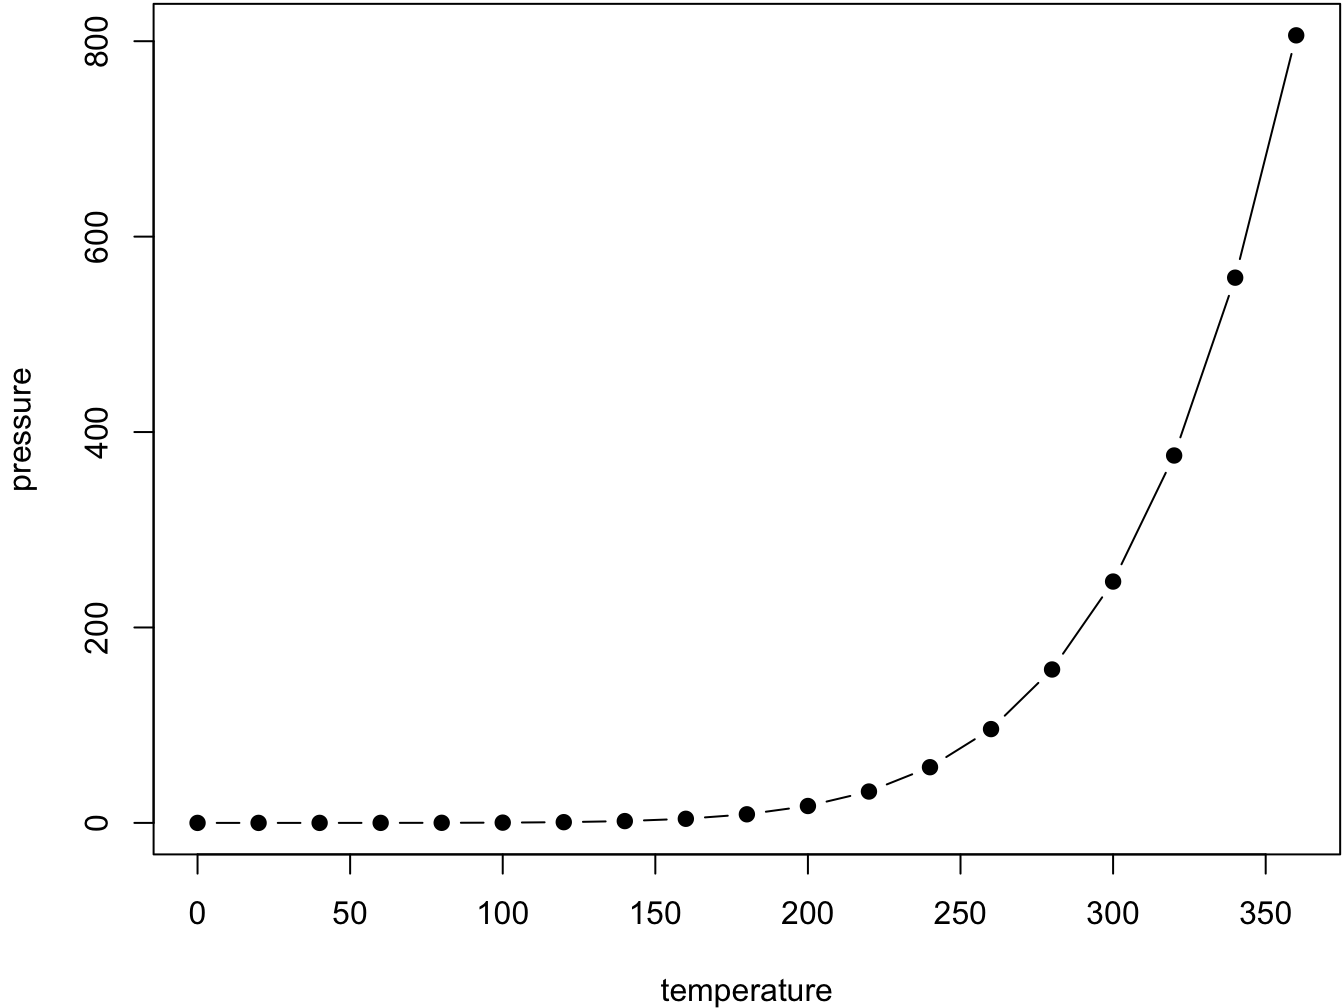
\includegraphics[width=0.8\linewidth]{bookdown-demo_files/figure-latex/nice-fig-1} 

}

\caption{Here is a nice figure!}\label{fig:nice-fig}
\end{figure}

Reference a figure by its code chunk label with the \texttt{fig:} prefix, e.g., see Figure \ref{fig:nice-fig}. Similarly, you can reference tables generated from \texttt{knitr::kable()}, e.g., see Table \ref{tab:nice-tab}.

\begin{Shaded}
\begin{Highlighting}[]
\NormalTok{knitr}\SpecialCharTok{::}\FunctionTok{kable}\NormalTok{(}
  \FunctionTok{head}\NormalTok{(iris, }\DecValTok{20}\NormalTok{), }\AttributeTok{caption =} \StringTok{\textquotesingle{}Here is a nice table!\textquotesingle{}}\NormalTok{,}
  \AttributeTok{booktabs =} \ConstantTok{TRUE}
\NormalTok{)}
\end{Highlighting}
\end{Shaded}

\begin{table}

\caption{\label{tab:nice-tab}Here is a nice table!}
\centering
\begin{tabular}[t]{rrrrl}
\toprule
Sepal.Length & Sepal.Width & Petal.Length & Petal.Width & Species\\
\midrule
5.1 & 3.5 & 1.4 & 0.2 & setosa\\
4.9 & 3.0 & 1.4 & 0.2 & setosa\\
4.7 & 3.2 & 1.3 & 0.2 & setosa\\
4.6 & 3.1 & 1.5 & 0.2 & setosa\\
5.0 & 3.6 & 1.4 & 0.2 & setosa\\
\addlinespace
5.4 & 3.9 & 1.7 & 0.4 & setosa\\
4.6 & 3.4 & 1.4 & 0.3 & setosa\\
5.0 & 3.4 & 1.5 & 0.2 & setosa\\
4.4 & 2.9 & 1.4 & 0.2 & setosa\\
4.9 & 3.1 & 1.5 & 0.1 & setosa\\
\addlinespace
5.4 & 3.7 & 1.5 & 0.2 & setosa\\
4.8 & 3.4 & 1.6 & 0.2 & setosa\\
4.8 & 3.0 & 1.4 & 0.1 & setosa\\
4.3 & 3.0 & 1.1 & 0.1 & setosa\\
5.8 & 4.0 & 1.2 & 0.2 & setosa\\
\addlinespace
5.7 & 4.4 & 1.5 & 0.4 & setosa\\
5.4 & 3.9 & 1.3 & 0.4 & setosa\\
5.1 & 3.5 & 1.4 & 0.3 & setosa\\
5.7 & 3.8 & 1.7 & 0.3 & setosa\\
5.1 & 3.8 & 1.5 & 0.3 & setosa\\
\bottomrule
\end{tabular}
\end{table}

You can write citations, too. For example, we are using the \textbf{bookdown} package \citep{R-bookdown} in this sample book, which was built on top of R Markdown and \textbf{knitr} \citep{xie2015}.

\hypertarget{elements-of-machine-learning}{%
\chapter{Elements of Machine Learning}\label{elements-of-machine-learning}}

In a minimalism style, machine learning refers to how computers can ``learn'' by finding patterns in data and using them to make predictions. Mathematically, given a real-valued output \(Y\) and predictors vector \(X\) containing \(p\) variables, we assume a general function \(f\) to describe \(Y\):

\begin{equation} 
Y = f(X) + \epsilon
\label{eq:ml01}
\end{equation}

Where, \(f\) is a fixed but unknown function, and \(\epsilon\) is a zero-mean random error term, which is supposed to be independent of \(X\).

The core of machine learning is a suite of data-driven algorithms for estimating \(f\). ML is based on {\emph{statistical learning theory}} to design models to understand patterns and employs {\emph{optimization algorithms}} to train the model to ``learn'' the pattern using input data.

The foundation of practical machine learning is the data. Data drives everything else. The model can not learn much pattern without enough data and could even have biased behaviour if the data quality is poor. In contrast, with substantial data, the machine learning model could achieve impressive results beyond expectation. A vivid example is to check the google's search engine - it is machine learning algorithm under the hood.

\begin{quote}
``All models are wrong, but some are useful.'' - George E.P. Box
\end{quote}

\hypertarget{linear-regression}{%
\section{Linear Regression}\label{linear-regression}}

Linear regression adopts a linear function\(f^{Linear}\) to equation \eqref{eq:ml01} with learnable model parameters \(B =(\beta_0,\beta_1,...,\beta_p) \in (p+1,1)\):

\begin{equation} 
Y = B^T X + \epsilon  
\label{eq:lm01}
\end{equation}

Here we assume the first column of \(X\) is all ones and thus \(\beta_0\) corresponds to the intercept term.

The model given by \eqref{eq:lm01} defines the {\emph{population regression line}}, which is the best linear approximation to the true relationship between \(X\) and \(Y\). The population regression line is unobserved and we have access to a set of sample observations to compute an sample-based estimate line. Fundamentally, we apply a standard statistical approach of using information from a sample to estimate characteristics of a large population. Here the linear regression focus on the estimate of coefficient \(\hat{B}\). The most popular estimation
method is {\emph{least squares}}.

Ordinary least square (OLS) regression is an estimated model based on sample data. We require a property of unbiasedness for estimator \(\hat{B}\). Unbiased estimator does not systematically over- or under-estimate the true parameter \(B\).

\[
\hat{B} = (X^TX)^{-1} X^T y
\]

\hypertarget{rethinking-the-unbiasedness-of-ols}{%
\subsection{Rethinking the Unbiasedness of OLS}\label{rethinking-the-unbiasedness-of-ols}}

Consider the decomposition of mean squared error of an estimator \(\tilde{\theta}\) in estimating \(\theta\):

\[
\begin{aligned}
MSE(\tilde{\theta}) &= E[ \tilde{\theta} - \theta ]^2 \\
                    &= Var( \tilde{\theta} ) +  [E( \tilde{\theta} ) - \theta ]^2
\end{aligned}
\]

Here the first term \(Var( \tilde{\theta} )\) is the variance, while the second term \([E( \tilde{\theta} ) - \theta ]^2\) is the squared bias.

The Gauss-Markov theorem implies that the least squares estimator has the smallest mean squared error (MSE) of all {\emph{linear estimators with no bias}} (⚠️ pay attention to the ``no bias'' here). However, there may well exist a biased estimator with smaller mean squared error. Such an estimator would {\emph{trade a little bias for a larger reduction in variance}}. Put bluntly, {\emph{biased estimates are commonly used}} for better out-of-sample performance (i.e., less MSE in test set). In reality, any method that shrinks or sets to zero some of the least squares coefficients may result in a biased estimate.

\hypertarget{assumptions-of-linear-model-and-violation-implications}{%
\section{Assumptions of Linear Model and Violation Implications}\label{assumptions-of-linear-model-and-violation-implications}}

\hypertarget{problem-1-non-linearity-of-the-data}{%
\subsection*{Problem 1: Non-linearity of the Data}\label{problem-1-non-linearity-of-the-data}}

The linear regression model assumes that there is a straight-line relationship between the predictors and the response. If the true relationship is far from linear, then all of the conclusions that we draw from the fit are suspect.

🔍 \emph{Residual plots} are a useful visualization tool for identifying non-linearity. Given a fitted linear regression model, we can plot the residuals, \(e_i = y_i - \hat{y_i}\), versus the predictor \(x_i\). In the case of a multivariate regression model, we can plot the residuals versus the fitted values \(\hat{y_i}\). Independence assumption implies no discernible pattern. The presence of a pattern may indicate a problem with some aspect of the linear model. For instance, if residuals exhibit a clear U-shape, which provides a strong indication of non-linearity in the data.

\hypertarget{problem-2-correlation-of-error-terms}{%
\subsection*{Problem 2: Correlation of Error Terms}\label{problem-2-correlation-of-error-terms}}

An important assumption of the linear regression model is that the error terms \({\epsilon_i}\) are uncorrelated. Intuitively, if the errors are uncorrelated, then the fact that \(epsilon_i\) is positive provides little or no information about the sign of \(\epsilon_{i+1}\). One counterexample is to think about double a set of training observations \((X, Y)\), as \(X_{Copy} = [X;X], Y_{Copy}=[Y;Y]\).

The standard errors that are computed for the estimated regression coefficients or the fitted values are based on the assumption of uncorrelated error terms. If in fact there is correlation among the error terms, then the estimated standard errors will tend to {underestimate} the true standard errors. As a result, confidence and prediction intervals will be narrower than expected.

Such residual correlations frequently occur in the context of {time series data}, which consists of observations for which measurements are obtained at discrete points in time. There is the issue of {residual \href{https://en.wikipedia.org/wiki/Autocorrelation}{autocorrelation}} - tracking in the residuals that adjacent residuals may have similar values.

In general, the assumption of uncorrelated errors is extremely important for linear regression as well as for other statistical methods, and good experimental design is crucial in order to mitigate the risk of such correlations.

\hypertarget{problem-3-outliers}{%
\subsection*{Problem 3: Outliers}\label{problem-3-outliers}}

An outlier is a point which is far from the value predicted by the model. Outliers can arise for a variety of reasons, such as incorrect data collection. They are quite common in real dataset.

Residual plots can be used to identify outliers. If we believe that an outlier has occurred due to an error in data collection, then one solution is to simply remove the observation. Shrewd care and revised assumptions should be taken when removing outliers, since an outlier may instead indicate a deficiency with the model, such as a missing predictor. 2008 global financial crisis is a data point that needs justification to be discarded as outlier.

\hypertarget{problem-4-collinearity}{%
\subsection*{Problem 4: 💥Collinearity}\label{problem-4-collinearity}}

Collinearity refers to the situation in which a group of variables are closely related to one another. The presence of collinearity can pose problems in the regression context, since it can be difficult to separate out the individual effects of collinear variables on the response. Collinearity reduces the accuracy of the estimates of the regression coefficients, it causes the standard error for \(\hat{\beta_j}\) to grow.

🔍 {Correlation matrix of the predictors} is a simple way to detect collinearity. Unfortunately, not all collinearity problems can be detected by inspection of the correlation matrix: it is possible for collinearity to exist between three or more variables even if no pair of variables has a particularly high correlation - this is called {\emph{multicollinearity}}.

There are in twp practical solutions to the problem of collinearity. The first, and more straightforward one, is to {drop} one of the problematic variables from the regression. The second solution is to aggregate the collinear variables together into a single composite predictor. For example, apply {\href{https://en.wikipedia.org/wiki/Principal_component_analysis}{PCA}} (Principal Component Analysis) approach to model the highly correlated features group and extract the first PC component as the representative indicator.

\hypertarget{conclusion}{%
\section{Conclusion}\label{conclusion}}

Linear models were largely developed in the precomputer age of statistics, but there are still robust baseline model to apply in today's computer era. They are simple and often provide an adequate and interpretable description of how the inputs affect the output. For prediction purposes they can sometimes outperform fancier nonlinear models, especially in situations with small numbers of training cases, low signal-to-noise ratio or sparse data.

\hypertarget{methods}{%
\chapter{Methods}\label{methods}}

We describe our methods in this chapter.

Math can be added in body using usual syntax like this

\hypertarget{math-example}{%
\section{math example}\label{math-example}}

\(p\) is unknown but expected to be around 1/3. Standard error will be approximated

\[
SE = \sqrt(\frac{p(1-p)}{n}) \approx \sqrt{\frac{1/3 (1 - 1/3)} {300}} = 0.027
\]

You can also use math in footnotes like this\footnote{where we mention \(p = \frac{a}{b}\)}.

We will approximate standard error to 0.027\footnote{\(p\) is unknown but expected to be around 1/3. Standard error will be approximated

  \[
  SE = \sqrt(\frac{p(1-p)}{n}) \approx \sqrt{\frac{1/3 (1 - 1/3)} {300}} = 0.027
  \]}

\hypertarget{applications}{%
\chapter{Applications}\label{applications}}

Some \emph{significant} applications are demonstrated in this chapter.

\hypertarget{example-one}{%
\section{Example one}\label{example-one}}

\hypertarget{example-two}{%
\section{Example two}\label{example-two}}

\hypertarget{final-words}{%
\chapter{Final Words}\label{final-words}}

We have finished a nice book.

  \bibliography{book.bib,packages.bib}

\end{document}
